\chapter{Maze complexity problems}\label{cha:background}
One of the main purposes of this thesis is to discuss the complexity of a maze. This chapter will provide a variety of maze and graph
complexity definitions which are implemented and compared in Chapter 5. Firstly the methods of complexity measure, derived from graph theory will be discussed followed by some existing concepts of measuring the complexity of a maze. Thinking about a maze and its complexity all different types of features and problems might be considered. 
It may be the difficulty of finding the way out, or difficulty of moving from point A to point B, or the difficulty of generating a particular maze. This chapter will provide a theoretical background for studying the maze complexity and in Chapter 5 detailed analysis based on examples will be provided. 
\section{Complexity measures in Graph Theory}
In this section approaches derived from graph theory, which describe and measure the complexity of a graph are presented.
 Conventionally, graph complexity in graph theory is evaluated by a degree distribution, a clustering coefficient, an edge density. Another approach derived from classical information theory is to generate graphs with some particularities while being random in all other aspects and then compare and decide whether a particular characteristic is typical among a group of graphs or not.
There is also a recent, advanced idea to use \textcolor{black}{a principle of maximum entropy} to estimate the algorithmic complexity of a graph. The main idea of the maximum entropy concept is that the more statistically random graph is, the more typical. \cite{11}. 
Studying the complexity of a graph is an important part of understanding it. By studying the complexity, we are acquiring knowledge about the system, how it could evolve, what are bottlenecks and variabilities, and how we can solve the problems posed by the system. Each application may understand the complexity differently. 
Each graph system, network and maze will cause different challenges and solutions to it. 
\subsection{Outlining Graph Parameters}
\begin{definition}\textbf{A Degree Distribution} \emph{\textcolor{red}{$P(k)$} is defined as a proportion of vertex with a degree $k$ to all vertices in a graph.}
\begin{equation}
P(k) = \frac{n_k}{n}
\end{equation}
\end{definition}
\begin{definition}\textbf{A Clustering Coeficient} \emph{$C_i$ is defined as a proportion of vertex links to vertex possible links. The coefficient for an undirected graph might be given by $C_i = \frac{k_i(k_i-1)}{2}$ where $k_i$ are the neighbours of vertex $v_i$. The average clustering coefficient is given by}
\begin{equation}
\bar{C} = \frac{1}{n}\sum_{n = 1}^{n} C_i
\end{equation}
\end{definition}
\begin{definition}\textbf{A Graph Entropy} “Graph entropy represents information-theoretic measures for characterizing networks quantitatively”\cite{12}.
\emph{It combines graph information and probabilistic distribution of vertices \cite{13}.}\end{definition}
\subsection{Shannon Entropy}
\textcolor{red}{An Adjacency matrix (Definition 3) of a maze may be also represented as a string. Adopting this, another maze complexity measure may be introduced.}
Shanon entropy derives directly from Boltzmann entropy in thermodynamics. “Shannon’s concept of information entropy quantifies the average number of bits needed to store or communicate a message.”\cite{11}. Studying complexity, the Shannon entropy measures how complex the string of a graph problem must be to avoid losing any information about its state. The main concept is that the information is built by $n$ different symbols and can not be stored in less than $log(n)$ bits.
Shanon entropy $H(M)$ of the object $M(R, p(x_i))$ is given by (4.3)\cite{11}:
\begin{equation}
H(M) = - \sum_{r = 1}^{r} p(x_i)\log_2 p(x_i)
\end{equation}
\textbf{Where:}\\
$R$ is a set of possible outcomes, e.g.  All possible adjacency matrix of size $m$\\
$p(x_i)$ is a probability of outcome $R$,\\
$r= |R|$\\
\section{Maze complexity Measures}
This section, summarize the characteristics which impact the complexity of a maze, such as maze size, average path length, density, and McClendon's complexity measure. It provides an overview of different approaches and tries to compare them. All parameters presented in this chapter are evaluated in Chapter 5.
\subsection{Independant Maze Parameters}
Size is one of the most indisputable complexity factors of a maze. A maze is described as per Definition 19. In Figure 4.1 two mazes with different sizes are
presented. It is almost too easy to think that a small maze is a simple maze, and a huge maze is a difficult one.\\
\begin{figure}[!h]
    \centering
    \begin{subfigure}{.5\textwidth}
    \centering
    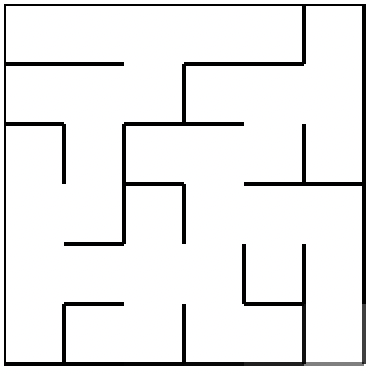
\includegraphics[width=.5\linewidth]{66}
    \caption{}
\label{fig:sub1}
    \end{subfigure}%
    \begin{subfigure}{.5\textwidth}
    \centering
    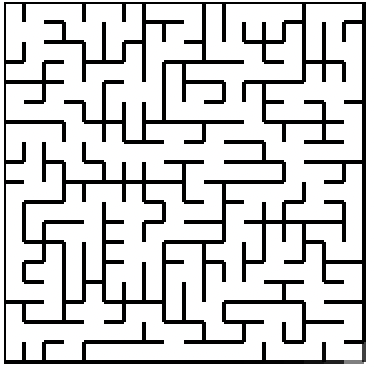
\includegraphics[width=.5\linewidth]{1818}
    \caption{}
\label{fig:sub2}
    \end{subfigure}
    \caption{Examples of different size mazes. Figure (a) it is an example of the Aldous-Broder maze of size 6 $\times$ 6, Figure (b) of size 18 $\times$ 18 \\ Source: Developed by the author, based on Aldous-Broder Algorithm Listing 1.2. }
\label{fig:test}
\end{figure}
\newline
Another key characteristic determining the complexity of a maze is the average length $\bar{p_l}$ of the paths in a maze. The longer the path, the bigger
the risk of following a faulty road to a solution. \textcolor{black}{Path is given by Definition 8}. Its beginning is always a start cell and it leads to
each dead-end in acyclic mazes. In cyclic mazes, paths can be infinite according to Definition 4. \textcolor{black}{In Figure 4.2 two mazes of the same size
but different average path lengths are presented}.
\newline
\begin{figure}[!h]
\centering
\begin{subfigure}{.5\textwidth}
\centering
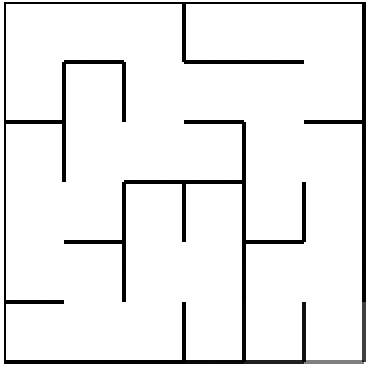
\includegraphics[width=.5\linewidth]{aldous}
\caption{}
\label{fig:sub1}
\end{subfigure}%
\begin{subfigure}{.5\textwidth}
\centering
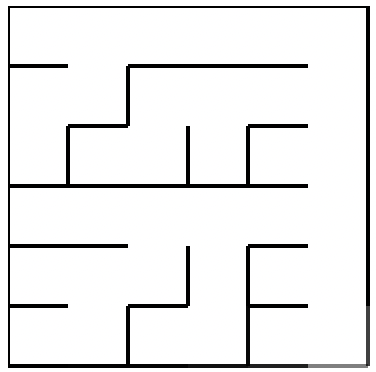
\includegraphics[width=.5\linewidth]{binary}
\caption{}
\label{fig:sub2}
\end{subfigure}
\caption{Examples of different average path length mazes. In figure (a) it s an example of the Aldous-Broder maze with $\bar{p}_l = 9.42$. Figure (b) it s an example of a Binary Tree maze with $\bar{p}_l = 10.8$\\ Source: Developed by the author,  based on Aldous-Broder Algorithm Listing 1.1 and Binary Tree Algorithm 1.2. }
\label{fig:test}
\end{figure}
Density for an acyclic graph is given by the equation (\ref{acyclic_density}), and density for a cyclic maze is given by the equation (\ref{cyclic_density}).
It describes the ratio between the number of all possible connections and the existing number of connections (edges).
\newpage
In Figure 4.3 two mazes with different
densities are presented.
\begin{figure}[!h]
\centering
\begin{subfigure}{.5\textwidth}
\centering
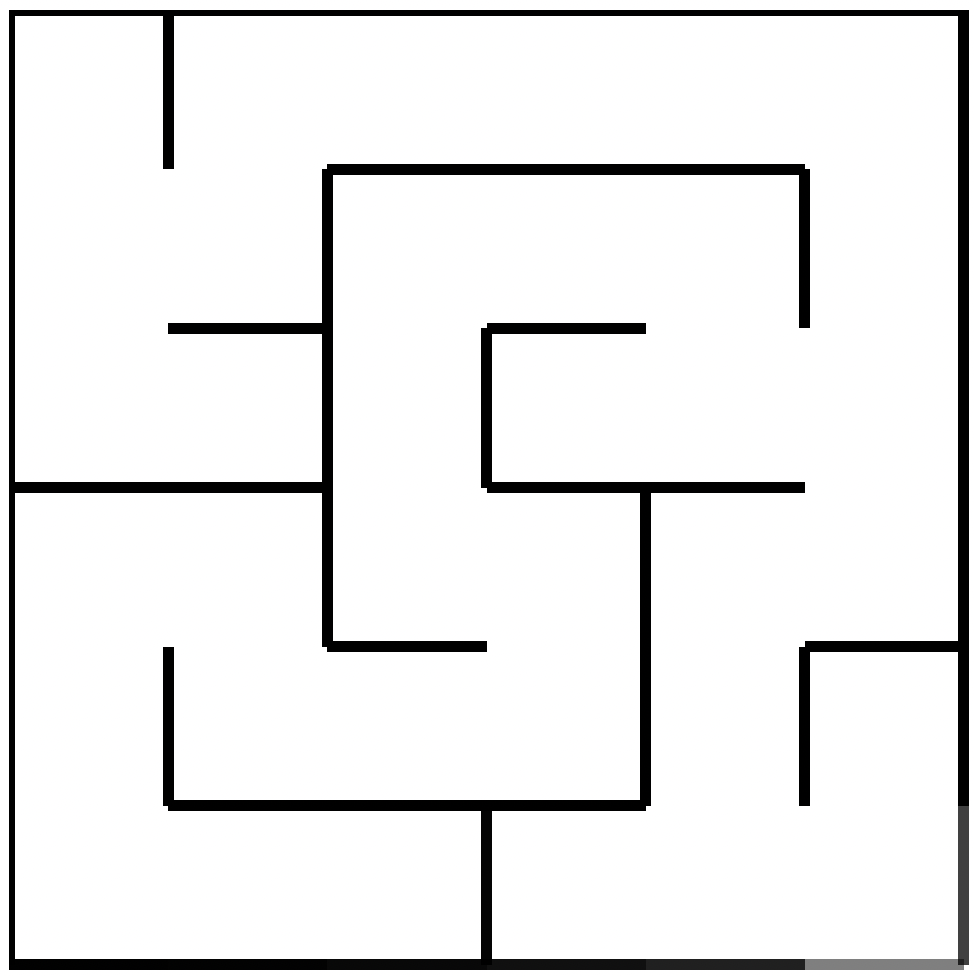
\includegraphics[width=.5\linewidth]{recursivedens}
\caption{}
\label{fig:sub1}
\end{subfigure}%
\begin{subfigure}{.5\textwidth}
\centering
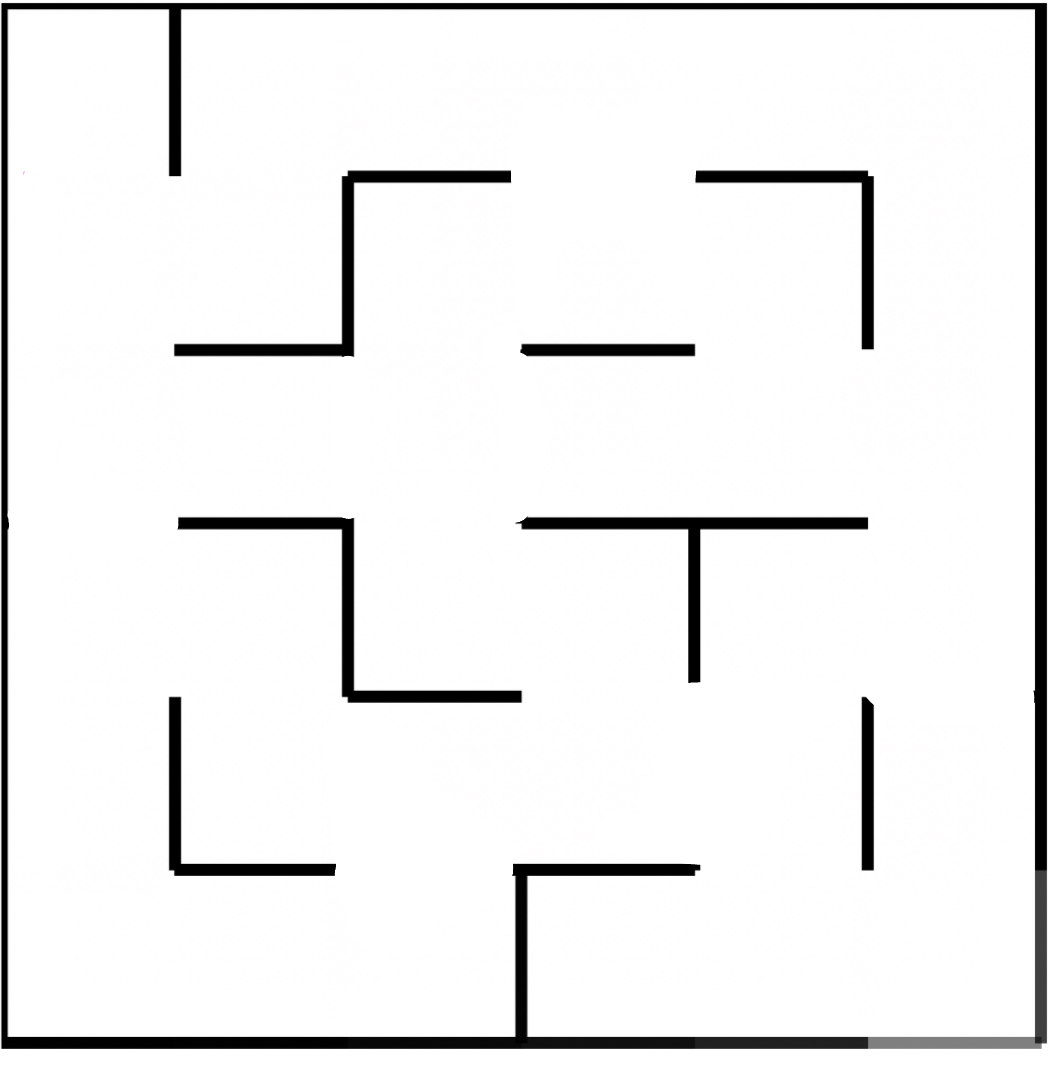
\includegraphics[width=.5\linewidth]{recursivedensecyclic}
\caption{}
\label{fig:sub2}
\end{subfigure}
\caption{Examples of different density mazes. In Figure (a) maze with density r $= 0.40$ is presented, and in Figure (b) maze with density r $ = 0.50$.\\Source: Developed by the author,  based on Aldous-Broder Algorithm Listing 1.1}
\label{fig:test}
\end{figure}

\newpage
\subsection{McClendon Measure}
Few sources are indicating a quantitative study of the measure of maze complexity. One of the most cited works in this field is a McClendon \textcolor{black}{\cite{14}} study of maze difficulty and complexity. 
McClendon’s work treats maze complexity and difficulty in a continuous measure using continuum theory. The main presuppositions of the work are that the maze is a perfect maze type and there are two distinguished pairs of points $(p,q)$ in the maze $M$ called gates. Where $p$ is an entrance and $q$ is an exit.  Hallways  $h$ build a maze. 
Where hallways are a subset $K$ of $M$ with the \textcolor{black}{$d(v) = 2$}. A subset $W_h = {w_1,w_2,\ldots, w_n}$ of $h$ incorporates all points of $h$. 
A trail is a path in the maze built by hallways. The branch is any trail intersecting the solution $S$ of a maze. Each branch in $M$ is connected to $S$ by a point $v_i$ in $I$ which is an intersections set $I = {v_1,v_2,\dots, v_n}$. The McClendon’s complexity of a hallway $h$ is given by:\\
\begin{equation}
\gamma(h) = D(h)\sum_{i = 1}^{i} \frac{\theta(w_i)}{d(w_i)\cdot \pi}
\end{equation}
\textbf{Where:}\\
$D(h)$ is an arclength of $h$,\\ 
$\theta(w_i)$ is the absolute value of the difference in the radian measures between the directions $V(t_i)$ and $V(t_{t+1})$\\ 
$d(w_i)$ is a length of a arc between $w_{i-1}$ and $w_i$ in $W_h$.\\ 
\newline
The McClendon’s complexity of a maze $M$ is given by:\\
\begin{equation}
\gamma(M)=\log\bigl[\gamma(S) + \sum_{i = 1}^{i} \gamma(B_i) \bigr]
\end{equation}
\textbf{Where:}\\
$\gamma(S)$ is a complexity of a solution of the maze,\\
$\gamma(B_j) = \sum_{i = 1}^{i} \gamma(h_i)$ is a complexity of a branch $B_j$.\\
\newline 
Using equation (4.5) requires knowledge about the solution of the maze. To avoid this, we should use the extrinsic approximation of the above method which is given by:\\
\begin{equation}
\gamma(M) \approx \log \bigl[\sum_{i =1}^{i}\gamma(h_i)\bigr]
\end{equation}
\\
\textbf{Where:}\\
$\gamma(h_i)$ is the complexity of an \textcolor{red}{$i^{th}$ hallway $h_i$}\\
 \newline
In this \textcolor{black}{thesis} we are using the square grid to generate and solve mazes. As a result of \textcolor{black}{a} uniform grid, the McClendon measure will be simplified, and calculated as:
\begin{equation} 
\gamma(M) \approx \log \bigl[\sum_{i =1}^{i}\frac{h(i)_l\cdot \mathcal{T}}{2}\bigr]
\end{equation}

\textbf{Where:}\\
$h(i)_l$ is the total length of the hallway,\\
$\mathcal{T}$ is the total number of L turns in the hallway, and each L turn is 90$^\circ$.%porownac to co wyjdzie z tym wykresem w tej pracy 
\subsection{Other approaches to delineate maze complexity }
In sections 4.1 and 4.2 different quantitative measures to define maze complexity were discussed. In this section, two descriptive methods determining the difficulty of the maze are presented. Biased mazes and the time complexity of maze generators may be considered as premises for reduced algorithmic randomness. This work will try to verify if those premises correlate with the time required to solve a maze, or it s McClendon’s complexity.\\ \newline
\textbf{Time Complexity of maze generators}\\
Looking at the time complexity of maze generators we can compare them and analyze whether the solution time depends on the time complexity. In Table 4.1 time complexity of different maze generators is presented. The analysis of the relation between time complexity and solution time is presented in Chapter 5.\\
\begin{table}[!ht]
\centering
\begin{tabular}{ |c||c| } 
\hline 
Maze Generator& Time Complexity\\ \hline
Binary Tree\cite{16} & $O(|V|)$\\
Aldous-Broder\cite{17}& $O(|V|^3)$\\ 
Recursive Backtracker\cite{18}& $O(|V|+|E|)$\\ 
\hline
 \end{tabular} 
\caption{Time complexity of maze generating algorithms, \textcolor{red}{represented in the Big O notation.\\Source: created by the author based on [16,17,18].}} 
 \end{table}
 \newline
 \newline
\textbf{Uniquness and Distinctiveness of a Maze}\\
Another approach to describing a maze might be evaluating its uniqueness and distinctiveness. For this purpose, it is possible to study how complicated the
algorithm generating a given maze must be and how statistically often a specific set of features occurs. One of the methods may be the parameterization of
the maze by classic measures such as density distribution or average path length and testing how often they appear in a specific configuration. Another
the method could be to look for biased features. Biased features are some peculiarities of the maze which are visible repeating structures. Good examples of a
biased maze might be a Binary Tree Algorithm, which tends to create visible diagonal intersections and two perpendicular corridors
at the edges of the maze presented in Figure 4.4(a). On the other hand, there are mazes generated with Aldous-Broder Algorithm, where no specific biases
occurs. \textcolor{red}{The unbiased texture of Aldous-Broder maze is visible in Figure 4.4(b)}.
\newline
\begin{figure}[!h]
    \centering
    \begin{subfigure}{.5\textwidth}
    \centering
    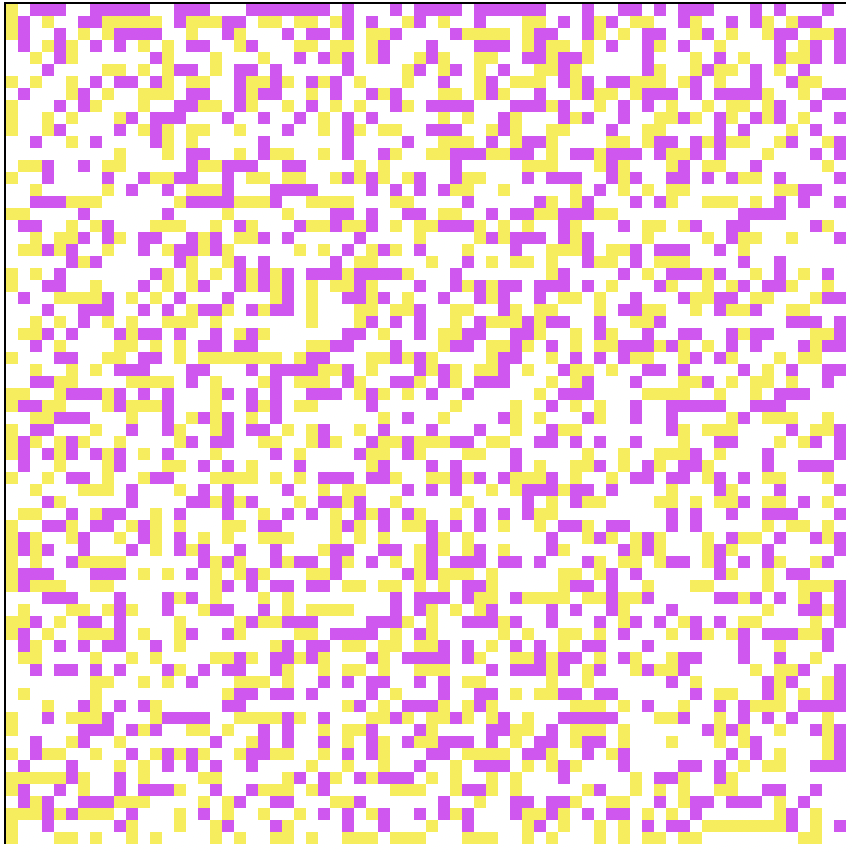
\includegraphics[width=.5\linewidth]{binarydegree.png}
    \caption{}
    \end{subfigure}%
    \begin{subfigure}{.5\textwidth}
    \centering
    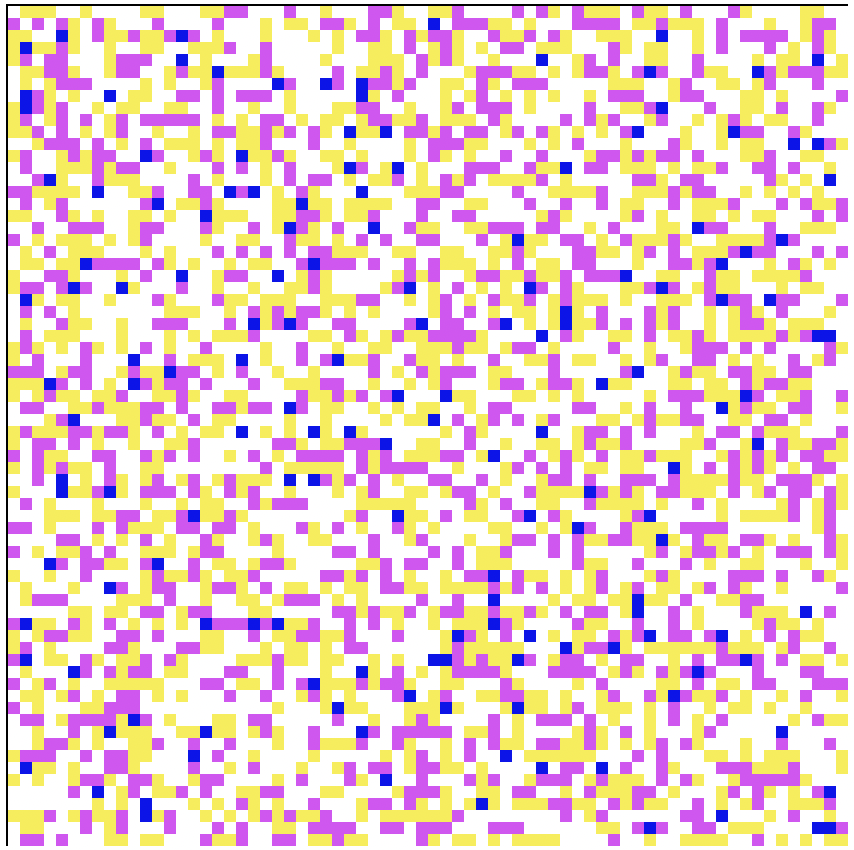
\includegraphics[width=.5\linewidth]{aldousdegree.png}
    \caption{}
    \end{subfigure}
    \caption{Examples of different textures in mazes. \textcolor{red}{Figure (a) and (b) present a degree distribution applied directly on a maze where all edges were removed.
    Each colour defines other cell degrees (Definition 11): yellow- a dead-end, white- a fork, pink- an intersection and blue- a cross}. In Figure (a) maze with a visible
    the diagonal texture was generated with Binary Tree Algorithm. In Figure (b) maze was generated with the Aldous-Broder Algorithm without any visible texture.\\Source: Mazes were generated by
    the author uses the algorithms described in Listings 2.1 and 2.2.}
    \end{figure}
